%% LaTeX-Beamer template for KIT design
%% by Erik Burger, Christian Hammer
%% title picture by Klaus Krogmann
%%
%% version 2.1
%%
%% mostly compatible to KIT corporate design v2.0
%% http://intranet.kit.edu/gestaltungsrichtlinien.php
%%
%% Problems, bugs and comments to
%% burger@kit.edu

\documentclass[18pt]{beamer}

%% SLIDE FORMAT

% use 'beamerthemekit' for standard 4:3 ratio
% for widescreen slides (16:9), use 'beamerthemekitwide'

\usepackage{templates/beamerthemekit}
% \usepackage{templates/beamerthemekitwide}

%% TITLE PICTURE

% if a custom picture is to be used on the title page, copy it into the 'logos'
% directory, in the line below, replace 'mypicture' with the
% filename (without extension) and uncomment the following line
% (picture proportions: 63 : 20 for standard, 169 : 40 for wide
% *.eps format if you use latex+dvips+ps2pdf,
% *.jpg/*.png/*.pdf if you use pdflatex)

\titleimage{lhc}

%% TITLE LOGO

% for a custom logo on the front page, copy your file into the 'logos'
% directory, insert the filename in the line below and uncomment it

\titlelogo{scc_logo}

% (*.eps format if you use latex+dvips+ps2pdf,
% *.jpg/*.png/*.pdf if you use pdflatex)

%% TikZ INTEGRATION

% use these packages for PCM symbols and UML classes
% \usepackage{templates/tikzkit}
% \usepackage{templates/tikzuml}

% the presentation starts here
\usepackage{caption}
\usepackage{subcaption}

\usepackage{tikz}
\usepackage{pgfplots}

\setbeamercovered{invisible}  % non transparent overlay

\title[rootJS]{rootJS - Specification}
\subtitle{PSE - Software Engineering Practice}
\author{C. Wolff, M. Fr\"uh, S. Rajgopal, C. Haas, J. Schwabe, T. Beffart}
%\author{Christoph Wolff, Maxi Fr\"uh, Sachin Rajgopal, Christoph Haas, Jonas Schwabe, Theo Beffart}

\institute{Steinbuch Center for Computing}

% Bibliography

\usepackage[citestyle=authoryear,bibstyle=numeric,hyperref,backend=biber]{biblatex}
\addbibresource{resources/references.bib}
\bibhang1em

\begin{document}

% change the following line to "ngerman" for German style date and logos
\selectlanguage{english}

%title page
\begin{frame}
\titlepage
\end{frame}

\section{PSE}

\begin{frame}{About PSE}
	Praxis der Softwareentwicklung(PSE) = Software Engineering Practice
	\begin{itemize}
		\item Waterfall model
		 \begin{itemize} 
			\item Planning/definition
		\end{itemize}
		\begin{figure}[htb]
		    \centering
		      \includegraphics[width=.80\textwidth, height=.80\textheight, keepaspectratio]{./resources/wasserfallmodell.png}
		      \nocite{swt:wfm}
		  \end{figure}
	\end{itemize}
\end{frame}

\section{Purpose}
\begin{frame}{Purpose}

\end{frame}

\chapter{Product usage}

ROOTjs will be used to create web-applications that can:
\begin{enumerate}
	\item Expose processed data (that might otherwise be hard to access) and then visualize it locally
	\item Interact with data both stored somewhere accessible for the server or streamed via RPC
	\item Run on any platform that supports a browser
\end{enumerate}


\section{Audience}
\begin{enumerate}
	\item particle physicists
	\item CERN
	\item Web-developers interested in creating applications based on ROOT
\end{enumerate}

\section{Operating conditions}

ROOTjs will be used on servers that run ROOT and have access to the required data sources.

\section{Product Environment}

\subsection{Software}
\begin{frame}{ROOT}
    \begin{itemize}
      \item process and visualize large amounts of scientific data (CERN)
      \item features a C++ interpreter (CLING) - i.e. used for rapid and efficient prototyping
      \item persistency mechanism for C++ objects
    \end{itemize}

    % \pause \kitbottom

  \begin{figure}[htb]
    \centering
    \begin{subfigure}[b]{0.5\textwidth}
           \includegraphics[width=0.97\linewidth, keepaspectratio]{./resources/root_application_domains.png}
           \nocite{cern:tut}
           %\caption{My Caption\footnotemark}
    \end{subfigure}%
    \begin{subfigure}[b]{0.5\textwidth}
          \includegraphics[width=0.97\linewidth, keepaspectratio]{./resources/root_application_domains2.png}
          \nocite{cern:domains}
    \end{subfigure}
  \end{figure}
  %\footnotetext{\cite{root_tut}}.}
\end{frame}

\begin{frame}{Node.js}

  \begin{itemize}
    \item open source runtime environment
    \begin{itemize}
        \item develop server side web applications
        \item act as a stand alone web server
    \end{itemize}

    \uncover<2->{
      \item Google V8 engine to execute JavaScript code
      \item rootJS bindings realized as native Node.js module written in C++
    }
  \end{itemize}

  \begin{figure}[htb]
    \centering
    \nocite{nodejs:logo}
  \end{figure}

\end{frame}

\subsection{Hardware}
\begin{frame}{Hardware}

\end{frame}

\chapter{Product data}



\begin{longtable}{|p{1cm} | p{15cm}|}
  \hline
  /D10/ & All ROOT classes and methods with corresponding signatures as they are dynamically mapped to JavaScript equivalents. They are also needed to support C/C++ specific features such as method overloading.\\
  \hline
  /D20/ & The ROOT environment state is preserved between calls from node.js. This means that objects and variables are available until the rootJS session has ended or a reset was explicitly triggered.\\
  \hline
  /D30/ & Application context deriving from TApplication, storing at least the correct program name and path\\
  \hline
\end{longtable}

\chapter{Product interface and functions}
The rootJS bindings will not have a user interface, neither a graphical user interface nor a command line interface.
This section will therefore specify the API of rootJS.


\begin{longtable}{|p{1cm} | p{15cm}|}
   \hline
  /I10/ & The module will expose a JavaScript object containing all accessible root variables, functions and classes \\
  \hline
  /I20/ & Exposed variables might contain scalar values, in this case they will be accessible in their JavaScript counterparts \\
  \hline
  /I30/ & Exposed variables might be objects, which are recursively converted to JavaScript objects until there are only scalar values \\
  \hline
  /I40/ & Exposed variables might be enums. In this case the identifier of the currently selected value is returned instead of the corresponding integer \\
  \hline
  /I50/ & Every exposed method will be accessible via a proxy method which handles parameter overloading, as JavaScript does not support overloading. If there is no method to handle the passed arguments, an exception will be thrown \\
  \hline
  /I55/ & A method can be called with an additional callback method that will be called after the original method has been executed \\
  \hline
  /I60/ & Exposed classes will be accessible as a constructor returning the object. The constructor will be proxied to support parameter overloading. If there is no method to handle the passed arguments, an exception will be thrown  \\
  \hline
  /I65/ & A constructor can be called with an additional callback method that will be called after the object has been constructed \\
  \hline
  /I70/ & The classes are encapsulated in their namespaces from ROOT. Each namespace is an Object containing namespaces or class constructors \\
  \hline
  /I80/ & Exceptions thrown by Root will be forwarded to JavaScript and can be treated by JavaScript as normal exceptions \\
  \hline
  /I90/ & Global variables are accessible via getter and setter methods to ensure their values are kept in sync with the ROOT framework \\
   \hline
\end{longtable}

\section{Scenarios}

Our bindings do not add to the core functionality of ROOT. Therefore 
we decided to give some examples on how the bindings might be used.

\begin{figure}[htb]
	\centering
	\begin{longtable}{p{3cm} @{\hskip 1cm} p{12cm}}
		\hline
		
		\textit{Scenario Name} & \underline{WebViewer}\\
		\hline
	
		\textit{Abstract} & A browser based GUI for realtime representation of root graphs.\\
		\hline
	
		\textit{Participating actor instances} & \underline{WebViewer:Node.js}; \underline{:ROOT}; \underline{:rootJS}\\
		\hline
	
		\textit{Flow of events} & 
		\begin{enumerate}
			\item rootJS is up and running initialize has already been executed.
			
			\item WebViewer calls the API method to get graphical output of the data ROOT has currently loaded.
				\begin{enumerate}
					\item rootJS processes the request and calls the corresponding ROOT functionality.
					\item rootJS receives ROOT output and streams it to WebViewer
				\end{enumerate}
			\item WebViewer uses the provided data to display the graph on its GUI
				\begin{enumerate}
					\item Node.js invokes ROOT I/O operations.
						\begin{enumerate}
							\item ROOT loads data and provides raw visualization data.
						\end{enumerate}
					\item Node.js serializes data and streams it to WebViewer.
				\end{enumerate}
			\item WebViewer receives data and renders it in the browser.
		\end{enumerate}
		\\
		\hline
		
	\end{longtable}
	
	\caption{WebViewer scenario}
	
\end{figure}

\begin{figure}[htb]
	\centering
	\begin{longtable}{p{3cm} @{\hskip 1cm} p{12cm}}
		\hline
		\textit{Scenario Name} & \underline{EventViewer}\\
		\hline
		\textit{Abstract} &
		A Web based event viewer providing a visualisation of experimental data, showing signals particles have produced in the detector.
		The web viewer is split into the back-end, server part, with access to
	    the data source and enough resources to process the data, and the front-end, client part, that is a modern-enough Web browser, and responsible only for visualisation itself and interaction with the user.
		\\
		\hline
		\textit{Participating actor instances} & 
		\underline{Server:Node.js Application}; \underline{:ROOT}; \underline{EventViewer:Browser}; \underline{:rootJS}\\
		\hline
		\textit{Flow of events} &
		\begin{enumerate}
			\item EventViewer requests visual updates from Server.
			\item Server interfaces with ROOT via rootJS.
			\item ROOT acquires data from external source.
			\begin{enumerate}
					\item External, dedicated readout hardware is used to access the data source.
					\item ROOT processes incoming data in a timely manner.
			\end{enumerate}
			\item ROOT passes the data prepared for (3D) visualisation to the Server via rootJS.
			\item Server publishes its data as JSON stream over the web.
			\item EventViewer renders received data locally e.g. using WebGL.
		\end{enumerate}
		\\
		\hline
	\end{longtable}
	\caption{EventViewer scenario}
\end{figure}

\subsection{Use Case 1: UseROOTConstant}

\begin{figure}[htb]
	\centering
	\begin{longtable}{p{3cm} @{\hskip 1cm} p{12cm}}
		\hline
		
		\textit{Use Case name} & \texttt{UseROOTConstant}\\
		\hline
		
		\textit{Participating actor instances} & Initiated by \texttt{NodeJSApplication}; Processed by \texttt{rootJS}; Communicates with \texttt{ROOT}\\
		\hline
		
		\textit{Flow of events} &
			\begin{enumerate}
				\item The \texttt{NodeJSApplication} requests access to a ROOT constant.
				\item \texttt{rootJS} sends a request to the corresponding ROOT constant.
				\item \texttt{ROOT} returns the requested value.
	                        \item The value is passed from \texttt{rootJS} to the \texttt{NodeJSApplication}.
			\end{enumerate}
			\\
		\hline
		
		\textit{Entry condition} & \texttt{rootJS} has been initialized\\
		\hline
		
		\textit{Exit condition} & The value has been returned to the NodeJSApplication\\
        \hline
	\end{longtable}
	
	\caption{Use Case: UseROOTConstant}
\end{figure}

\section{System Model}
\subsection{Initialization}
\begin{frame}{Initialization}
  \begin{itemize}
    \item Expose all
    \begin{itemize}
      \item Global variables
      \item Global functions
      \item Classes
    \end{itemize}
    \pause
    \item Each are bound to corresponding proxy methods
    \item An object which members are the exposed features is beeing passed to node
  \end{itemize}
  \pause
  \begin{block}{Names}
    \begin{itemize}
      \item Functions and classes have the same name as in Root
      \item Global variables can be called using Get[Variable] and Set[Variable] methods
    \end{itemize}
  \end{block}
\end{frame}

\subsection{Call a feature}
\begin{frame}{Call a feature}
  \begin{itemize}
    \item All features in node are mapped to a proxy method that will be called
    \pause
    \item The proxy method will eventually call a root function and pass the result to our ObjectFactory
    \pause
    \item By looking at the object type an corresponding v8::Handle will be generated and returned to node
    \begin{itemize}
      \item If the result is an object this will be done recursively
    \end{itemize}
  \end{itemize}
\end{frame}

\chapter{Global Test Cases}
During the development process continuous integration tools will be used to run at least the following test cases: \\

\begin{longtable}{|p{1cm} | p{15cm}|}
  \hline
  /T10/ & Read all global variables.\\
  \hline
  /T20/ & Write to all global variables that are not constant.\\
  \hline
  /T30/ & Write to all global variables that are constant and ensure the correct Exception is thrown.\\
  \hline
  /T40/ & Create instances of all classes with a public constructor.\\
  \hline
  /T50/ & Call all methods of these objects with valid parameters, where valid means that the data type is correct, a method throwing an exception due to invalid input shall be considered as a passed test, a crash due to e.g. invalid memory read shall be considered as a failed test.\\
  \hline
  /T60/ & Read all public member variables of these classes.\\
  \hline
  /T70/ & Write to all public member variables of these classes that are not constant.\\
  \hline
  /T80/ & Write to all public member variables of these classes that are constant and ensure the correct exception is thrown.\\
  \hline
  /T90/ & Create instances of classes with private constructors and ensure the correct exception is thrown.\\
  \hline
  /T100/ &  Apply the test cases described in /T60/ to /T90/ to static members and methods. Ensure the correct exceptions are thrown.\\
  \hline
  /T110/ & Let Cling evaluate strings of valid C++ code during run time and ensure ROOT's state wad modified as expected.\\
  \hline
  /T120/ & Let Cling evaluate strings of syntactically invalid C++ code during run time and ensure the right exceptions are thrown and forwarded correctly.\\
  \hline
  /T130/ & Let Cling evaluate strings of semantically invalid C++ code during run time and ensure the right exceptions are thrown and forwarded correctly.\\
  \hline
\end{longtable}

\section{Statistics}

\begin{frame}{Merges}
        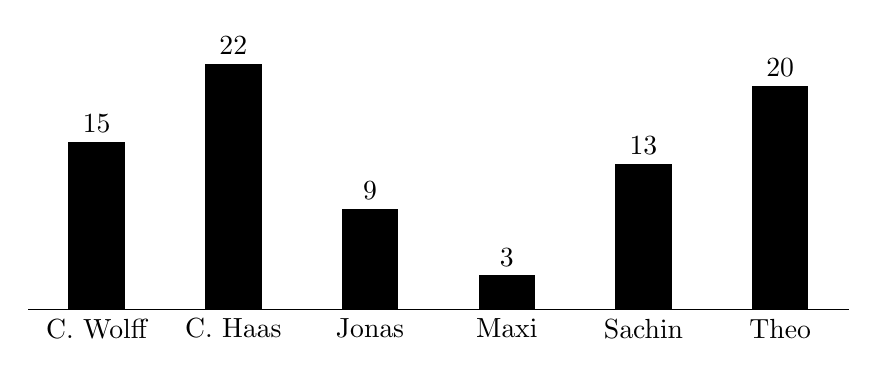
\begin{tikzpicture}
                \begin{axis}[
                     width  = 12cm,
                     hide y axis,
                     axis x line*=bottom,
                     height = 5cm,
                     bar width=20pt,
                     symbolic x coords={C. Wolff, C. Haas, Jonas, Maxi, Sachin, Theo},
                     nodes near coords,
                     ymin=0
                     ]
                     \addplot[ybar, fill=black] coordinates {
                          (C. Wolff,15)
                          (C. Haas,22)
                          (Jonas,9)
                          (Maxi,3)
                          (Sachin,13)
                          (Theo,20)
                     };
                \end{axis}
        \end{tikzpicture}
        \end{frame}

\begin{frame}{Punchcard}
        \includegraphics[keepaspectratio,width=12cm]{./resources/punchcard.png} 
\end{frame}
        


\appendix
\beginbackup

\begin{frame}[allowframebreaks]{References}
\printbibliography
\end{frame}

\backupend

\end{document}
